% !TEX TS-program = pdflatex
% !TEX encoding = UTF-8 Unicode

% Example of the Memoir class, an alternative to the default LaTeX classes such as article and book, with many added features built into the class itself.

\documentclass[12pt,a4paper,oneside,obeyspaces]{memoir} % for a long document
% \documentclass[12pt,a4paper,article]{memoir} % for a short document
\usepackage[utf8]{inputenc} % set input encoding to utf8
\usepackage[hidelinks]{hyperref}
\usepackage{listings}
\usepackage{longtable}
\usepackage{cleveref}
\usepackage{graphicx}
\usepackage{amsmath}
\usepackage{color}
\usepackage{booktabs}
\usepackage[table]{xcolor} % to highlight table rows
\usepackage{url} % for typesetting file paths
\usepackage{siunitx} % for units

% Don't forget to read the Memoir manual: memman.pdf

\definecolor{highlightcolor}{rgb}{.95,.95,1.0} % highlight color for table rows
\definecolor{lstcolor}{rgb}{.95,.95,0.95} % background color for listings

% set the options for listing
\sbox0{\small\ttfamily A}
\edef\mybasewidth{\the\wd0 }
\lstset{
    basicstyle=\small\ttfamily,% print whole listing small
    columns=fixed,
    basewidth=\mybasewidth,
    breaklines=true, % break lines
    postbreak=\raisebox{0ex}[0ex][0ex]{\ensuremath{\color{red}\hookrightarrow\space}}, % add a red arrow at new broken line
    backgroundcolor=\color{lstcolor}, % background color of listing box
    framexleftmargin=6pt, % padding
    framextopmargin=6pt, % padding
    framexrightmargin=6pt, % padding
    framexbottommargin=6pt, % padding
    frame=tb, framerule=0pt, % padding
}
\newsavebox\lstbox

% set up appendix
\renewcommand*{\cftappendixname}{Appendix\space}

% set up command to stretch table height
\newcommand{\ra}[1]{\renewcommand{\arraystretch}{#1}} 

% set up command for degree fahrehnheit
\DeclareSIUnit\Fahrenheit{\degree F}

%%% Examples of Memoir customization
%%% enable, disable or adjust these as desired

%%% PAGE DIMENSIONS
% Set up the paper to be as close as possible to both A4 & letter:
\settrimmedsize{11in}{210mm}{*} % letter = 11in tall; a4 = 210mm wide
\setlength{\trimtop}{0pt}
\setlength{\trimedge}{\stockwidth}
\addtolength{\trimedge}{-\paperwidth}
\settypeblocksize{22cm}{16cm}{*}
\setulmargins{*}{*}{*} % 50pt upper margins
\setlrmargins{*}{*}{1} % set the margins to be equal
\checkandfixthelayout

% This is from memman.pdf

%%% ToC (table of contents) APPEARANCE
\maxtocdepth{subsection} % include subsections
\renewcommand{\cftchapterpagefont}{}
% \renewcommand{\cftchapterfont}{}     % no bold!

%%% HEADERS & FOOTERS
\pagestyle{ruled} % try also: empty , plain , headings , ruled , Ruled , companion

%%% CHAPTERS
\chapterstyle{hangnum} % try also: default , section , hangnum , companion , article, demo

\renewcommand{\chaptitlefont}{\Huge\sffamily\raggedright} % set sans serif chapter title font
\renewcommand{\chapnumfont}{\Huge\sffamily\raggedright} % set sans serif chapter number font

%%% SECTIONS
\hangsecnum % hang the section numbers into the margin to match \chapterstyle{hangnum}
\maxsecnumdepth{subsection} % number subsections

\setsecheadstyle{\Large\sffamily\raggedright} % set sans serif section font
\setsubsecheadstyle{\large\sffamily\raggedright} % set sans serif subsection font

%% END Memoir customization

%%% BEGIN DOCUMENT
\begin{document}

% set bib style
\bibliographystyle{plain}

% render titlepage
%!TEX root = ../User Guide.tex
\begin{titlingpage}
\clearpage\thispagestyle{empty}

\begin{center}
 {\sffamily\huge CACTUS User Guide\\}
 % ----------------------------------------------------------------
 \vspace{1.5cm}
 {\Large Jonathan C. Murray \\ Aerosciences Department}\\[5pt]

 \vspace{1.5cm}
 {\Large Matthew Barone \\ Wind Energy Technologies}\\[5pt]

 \vspace{1.5cm}
 {\Large Phillip K. Chiu \\ Wind Energy Technologies}\\[5pt]
  % ----------------------------------------------------------------
 \vspace{8cm}
{\Large Sandia National Laboratories \\
P.O. Box 5800 \\
Albuquerque, NM 87185 \\}
 % ----------------------------------------------------------------
 \end{center}
 \end{titlingpage}

\tableofcontents % the asterisk means that the contents itself isn't put into the ToC
\listoffigures
\listoftables

\cleartorecto % new page before the first chapter
\ra{1.3} % set the table row spacing for all chapters
%!TEX root = ../User Guide.tex
\chapter{Introduction and overview}
CACTUS (\textbf{C}ode for \textbf{A}xial and \textbf{C}rossflow \textbf{TU}rbine \textbf{S}imulation) is a turbine performance simulation code using a blade element discretization and a free vortex line description of the turbine wake. The code was originally based on \texttt{VDART3}, a free vortex wake simulation of the Darrieus wind turbine, developed by Strickland \cite{Strickland1979}. The codebase has been largely upgraded to the Fortran 9x standard, and a number of modifications have been made to the original \texttt{VDART3} methods including updates to the blade loads models, and new models to handle generic device geometry and marine turbine specific physics.

This document serves as a user's manual for CACTUS. A brief overview of the code is provided below, however, more detailed information on the methods used can be found in \cite{Murray2011}. 

\section{Blade loads and wake models}
CACTUS simulates a turbine device consisting of an arbitrary configuration of blade element sections. Each section can be assigned arbitrary load coefficient vs. angle of attack characteristics, which typically correspond to two-dimensional lift and drag coefficient data for a particular foil section. Since data from two-dimensional wind tunnel tests or foil performance calculations are used to represent element loads, it is generally assumed that these elements are in locally two-dimensional flow. 

A rotor blade consisting of an arbitrary planform shape and foil sections can be modeled by the synthesis of a number of blade elements. The blade loads and wake of the turbine rotor are evolved in time over a certain number of rotor revolutions, until the revolution-averaged rotor power is converged.  The code output includes the blade aerodynamic forces, wake vortex trajectories, and performance metrics such as torque and power.  

CACTUS uses a potential flow model comprised of free vortex line elements to represent the turbine wake flow field. The vortex line structure attached to a single blade element is shown in \Cref{fig:vortex_lattice}. At each point in time, the bound vorticity ($\Gamma_B$) on each blade element is related to the element lift coefficient through the Kutta-Joukowski theorem, and the spanwise ($\Gamma_S$) and trailing vorticity ($\Gamma_T$) are recovered through the application of the Helmholz theorem of conservation of circulation along a vortex line \cite{katz2001low}.

\begin{figure}
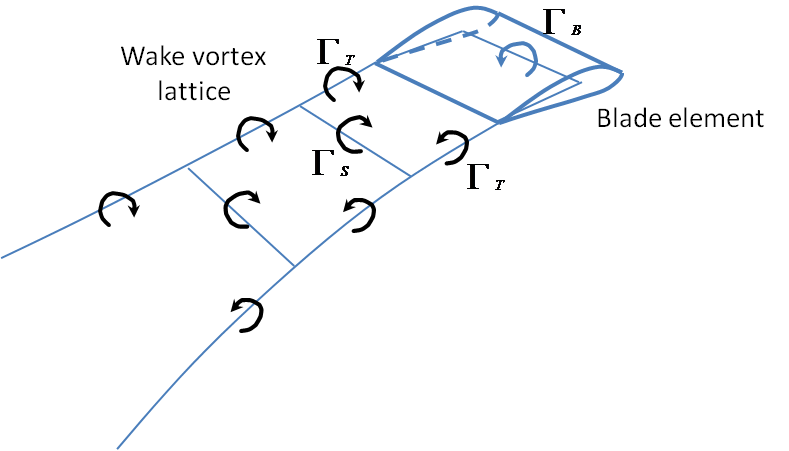
\includegraphics{figures/vortex_lattice.png}
\label{fig:vortex_lattice}
\caption{Blade element with associated vortex lattice system.}
\end{figure}

\subsection{Dynamic blade loads}
The operational cycle of some turbines, most notably cross-flow turbines or axial flow turbines in yawed flow conditions, cause the turbine blades to operate in dynamically variable flow conditions. The effects of blade rotation with respect to the surrounding fluid and the effects of dynamically variable flow angle of attack are captured with additional models.

The effects of blade section pitch rate (rotation around an axis normal to the section plane) are captured by analogy to an analytical solution for a pitching flat plate. Improvements have been made to the original methodology used in \texttt{VDART3}, and modifications have been made to handle non-zero section pitching moment due to cambered foil sections.

Under certain operational conditions, the turbine blades may operate at angles of attack beyond their steady-state stall limits for significant lengths of time. The transient behavior of the blade section loads during this ``dynamic stalling'' process must be modeled as it is not captured by the steady load coefficient data input for each foil section. The primary effect of dynamic stalling is a delay in the appearance of stalled flow effects on blade loads to higher angles of attack than would be expected in steady flow.

Two models for dynamic stall effects on blade section loads are included in CACTUS. The modified Boeing-Vertol method of Gormont is the default. This algebraic method approximates dynamic stall effects with a ``lagged'' angle of attack, where the magnitude of the lag is empirically correlated to the angle of attack rate. The Leishman-Beddoes model incorporates more physical models and attempts to model the temporal evolution of dynamic stall flow phenomena and associated effects on blade loads. This model may provide more accurate results than the algebraic Boeing-Vertol method, but requires many more simulation time steps to be taken per turbine revolution to achieve converged results.

\section{Wall boundaries}
CACTUS can simulate the effects of proximity to a ground plane or free (water) surface on turbine performance. The boundary conditions, either zero normal flow for a ground plane or constant surface pressure for a free surface, are applied using rectangular source panel elements. The free surface boundary condition is currently implemented as a quasi-static boundary, allowing it to respond only to the average flow created by the turbine and wake over a full revolution. 

The user is allowed to specify the time step interval between updates to the wall panel system. For the free surface model, the wall update interval specifies the number of time steps between updates to the revolution averaged quantities. It is often not necessary to update these quantities on every time step. If it's possible to reduce the frequency of wall panel system updates and still obtain convergence of the simulation output of interest, this can reduce simulation run time considerably.
%!TEX root = ../User Guide.tex
\chapter{Normalization parameters}
Some definitions of parameters used in normalize CACTUS input and output parameters are given in \Cref{tbl:normalization_parameters}.

\begin{table}[!htbp]
\centering
\caption{Parameters used for non-dimensionalization.}
\label{tbl:normalization_parameters}
\begin{tabular}{p{0.20\textwidth}p{0.70\textwidth}}
\toprule
Variable          & Description \\
\midrule
$\rho$            & Fluid density \\
$U_\infty$        & Freestream fluid flow speed \\
$A_T$             & Turbine reference area. Typically this reference area is chosen to be the projected frontal area of the volume swept by the rotor. \\
$R$               & Turbine reference radius \\
$\omega$          & Turbine rotation rate \\
$U_\textrm{local}$& Fluid flow speed local to an element. \\
$U_\textrm{tip}$  & Turbine tip speed. Defined as $U_\textrm{tip} = \omega R$. \\
$c$               & Element chord length \\
$A_E$             & Element planform area \\
\bottomrule
\end{tabular}
\end{table}

In general, most parameters have been normalized at the machine scale. Unless otherwise noted in the input and output descriptions below, the force, torque, and power coefficients are normalized as:

$$ C_F = \frac{F}{\frac{1}{2} \rho U_\infty^2 A_T} $$
$$ C_T = \frac{T}{\frac{1}{2} \rho U_\infty^2 A_T R} $$
$$ C_P = \frac{P}{\frac{1}{2} \rho U_\infty^3 A_T} $$
%!TEX root = ../User Guide.tex
\chapter{Input files}
This section describes the namelist, geometry, and airfoil data input files required by CACTUS. CACTUS is run from the command line with the path to the namelist input file passed as the only argument. The geometry input file and the airfoil data table files are referenced in the namelist input file.

\section{CACTUS namelist input}
This section describes the FORTRAN namelist input file for CACTUS. There are two namelist groups in the input file, \path{\&ConfigInputs} and \path{\&CaseInputs}. The parameters that can be input in each group are given in the tables below. Parameters not specified in the namelist input are left at the indicated default values. The parameters listed in bold font below are the parameters most commonly specified in an input file (with the rest being left at default values). 
\subsection{Input configuration}

\begin{longtable}{p{0.20\textwidth}p{0.70\textwidth}}
\caption{Available input configuration options in the \texttt{\&ConfigInputs} namelist.} \label{tbl:configinputs} \\
\multicolumn{2}{c} {\emph{Regression testing}}  \\ \toprule
Variable name & Description \\ \midrule
\path{RegTFlag}             & Set to 1 to perform a regression test (two iterations, generates \path{_RegData.out} output file), 0 for normal operation (default). \\
\bottomrule
\\
\multicolumn{2}{c} {\emph{Wall calculation}}  \\ \toprule
Variable name & Description \\ \midrule
\path{GPFlag}               & Set to 1 to use a ground plane, 0 otherwise (default 0). \\ 
\path{FSFlag}               & Set to 1 to use a free surface, 0 otherwise (default 0). \\ 
\path{GPGridSF}             & Factor on default ground plane grid spacing (default 1). \\ 
\path{FSGridSF}             & Factor on default free surface near-field grid spacing (default 1). \\ 
\path{GPGridExtent}         & Distance the ground plane will extend from the turbine location. Measured in rotor radii. (default 10.0) \\ 
\path{WPFlag}               & Set to 1 to use a wall geometry read in from file, 0 otherwise (default 0). \\
\bottomrule
\\
\multicolumn{2}{c} {\emph{Calculation inputs}}  \\ \toprule
Variable name & Description \\ \midrule
\path{nr}                   & Number of revolutions to perform (default 10) \\ 
\path{nti}                  & Number of time steps per revolution (default 20) \\ 
\path{convrg}               & Convergence level for the revolution average power coefficient. Iteration will finish before nr revs if this level is hit. Input -1 to skip convergence check (default). \\ 
\path{iut}                  & Number of iterations between wake convection velocity updates. If set to zero, the interval will be calculated automatically. If negative, wake convection velocities will be left at the values calculated at the time the wake element is created (no wake convection velocity updates). \\ 
\path{iWall}                & Number of iterations between wall model updates (if wall calculation is active). \\ 
\path{TSFilFlag}            & Flag to enable timestep filtering. Set to 1 to enable filtering of the blade bound vorticity smooth over ntsf timesteps (often needed for stability when blade chord to radius ratio is high). Set to 0 for no filtering (default). \\ 
\path{ntsf}                 & Number of timesteps over which the blade bound vorticity is filtered smooth when \path{TSFilFlag} = 1 (default 3). \\ 
\path{ivtxcor}              & Flag to specify the finite vortex core model to use. Input 1 for constant vorticity in the core (default). Input 2 to use linear radial vorticity distribution in core. Input 0 to turn off core model. \\ 
\path{vcrfb}                & Factor on nominal bound vortex core radius used if \path{ivtxcor = 1} (default 1). Nominal bound vortex core radius is specified by the maximum blade chord value input in the turbine geometry specification. \\ 
\path{vcrft}                & Factor on nominal trailing wake vortex core radius used if \path{ivtxcor = 1} (default 1). Nominal trailing wake vortex core radius is specified by the maximum blade element span value input in the turbine geometry specification. \\ 
\path{vcrfs}                & Factor on nominal spanwise wake vortex core radius used if \path{ivtxcor = 1} (default 1). Nominal spanwise wake vortex core radius is calculated from a reference distance between spanwise wake lines given the temporal discretization level used. \\ 
\path{vcutoffrad}           & Cutoff radius used for vortex induced velocity calculation (default \num{1.0e-7}). \\ 
\path{Incompr}              & 1 to ignore any compressibility effects in models, 0 to include compressibility effects (default). \\ 
\path{ifc}                  & 1 to use final convergence step, 0 to not (default). If selected, the temporal discretization level is refined once/if initial convergence is reached before nr revolutions have been performed. \\ 
\path{nric}                 & Revolution number after which to switch to final convergence, if initial convergence level has not yet been achieved. Input -1 to skip this check (default). \\ 
\path{ntif}                 & Final number of time steps per revolution. This value will replace \path{nti} during final convergence. Input -1 to leave \path{ntif = nti} (default). \\ 
\path{convrgf}              & Final convergence level. This level will replace \path{convrg} during final convergence. Input -1 to skip final convergence check (default). \\ 
\path{iutf}                 & Final number of iterations between wake updates. This value will replace \path{iut} during final convergence. Default behavior is the same as \path{iut}. \\ 
\path{ixterm}               & 1 to ignore wake points beyond $x/R =$ \path{xstop}, 0 to use all wake points (default). \\ 
\path{xstop}                & If \path{ixterm = 1}, defines $x/R$ beyond which wake points are ignored (default 5) \\ 
\bottomrule
\\
\multicolumn{2}{c} {\emph{Unsteady aerodynamics}}  \\ \midrule Variable name & Description \\ \midrule
\path{DSFlag}               & 0 for no dynamic stall, 1 for Modified Boeing-Vertol model (default), 2 for Leishman-Beddoes model. \\ 
\path{PRFlag}               & 0 for no element pitch rate aerodynamic effects, 1 to include these effects (default). \\ 
\bottomrule
\end{longtable}

\subsection{Case inputs}

\begin{longtable}{p{0.20\textwidth}p{0.70\textwidth}}
\caption{Available input configuration options in the \texttt{\&CaseInputs} namelist.} \label{tbl:caseinputs} \\
\multicolumn{2}{c} {\emph{Operation point inputs}}  \\ \toprule
Variable name & Description \\ \midrule
\path{RPM}         & Rotor rotation rate (revs per minute). \\
\path{Ut}          & Tip speed ratio with freestream flow speed ($U_\textrm{tip}/U_\infty$) \\
\path{rho}         & Density (\si{slug/ft^3}) \\
\path{vis}         & Dynamic viscosity (\si{slug/(ft.s)}) \\
\path{tempr}       & Temperature (\si{\Fahrenheit}) \\
\path{hBLRef}      & Height above ground of the effective freestream to be used in ground shear layer model (ft). \\
\path{slex}        & Exponent for ground shear layer model (Ex. 1/2 for parabolic laminar BL model, 1/7 turbulent approx., 0 for constant freestream). \\
\path{hAG}         & Height above ground at turbine geometry origin point (\si{ft}). Note that the ground plane is assumed to be oriented with its normal vector in the +$y$ direction. \\
\path{dFS}          & Depth below un-deflected free surface of the turbine geometry origin point (\si{ft}). Only used if free surface calculation is active. Note that the un-deflected free surface is assumed to be oriented with its normal vector in the +$y$ direction. \\
\path{igust}        & 1 to activate sinusoidal gust model, 0 to use nominal constant freestream model (default). The sinusoidal gust perturbation is modeled per the IEC 61400-1 Wind Turbine Design Standard. \\
\path{gustamp}     & Amplitude of sinusoidal gust perturbation (m/s) used if \path{igust} = 1. \\
\path{gusttime}    & Timescale of sinusoidal gust perturbation (s) used if \path{igust} = 1. \\
\path{gustX0}      & Starting x location of the gust divided by reference radius (location where perturbation is zero at initial simulation time). Used if igust = 1. \\
\path{itower}      & 1 to activate the tower wake model, 0 otherwise (default). This model adds an empirically defined viscous wake deficit to the nominal freestream to model the presence of the support tower. The model currently assumes this tower to be oriented along the y-axis. \\
\path{tower_Npts}  & Number of elements used to represent the tower (default 10). \path{itower} = 1. \\
\path{tower_x}     & Tower location x coordinate divided by reference radius. Used if \path{itower} = 1. \\
\path{tower_ybot}  & Lower tower y coordinate divided by reference radius. Used if \path{itower} = 1. \\
\path{tower_ytop}  & Upper tower y coordinate divided by reference radius. Used if \path{itower} = 1. \\
\path{tower_D}     & Tower diameter divided by reference radius. Used if \path{itower} = 1. \\
\path{tower_CD}    & Tower 2D sectional drag coefficient based on tower diameter (default 1.0). Used if \path{itower} = 1. \\
\bottomrule
\\
\multicolumn{2}{c} {\emph{Geometry and airfoil data}}  \\ \toprule
Variable name & Description \\ \midrule
\path{GeomFilePath} & (string in single quotes) Path to turbine geometry input file. \\
\path{nSect}        & Number of airfoil section data tables to use (default 1). \\
\path{AFDPath}      & (string in single quotes) Array (comma separated) of section data file path strings (size=nsect). \\
\path{AFDPath}      & (string in single quotes) Array (comma separated) of section data file path strings (size=nsect). \\
\path{WallMeshPath} & (string in single quotes) Path to wall mesh file in Plot3D format. Only read if \path{WallFlag} = 1. \\
\bottomrule
\\
\multicolumn{2}{c} {\emph{Other parameters}}  \\ \toprule
Variable name & Description \\ \midrule
\path{Jbtitle}     & (string in single quotes) Job title. \\
\path{CDPar}       & Additional parasitic interference drag coefficient based on ``chord area'' (chord squared) to be applied to the blade/strut interference drag calculation (default 0). \\
\path{CTExcrM}     & Additional machine level excrescence torque coefficient, specified by $C_{T,\textrm{ExcrM}} = T_\textrm{ExcrM}/\frac{1}{rho} U_\textrm{tip}^2 R^3$ (default 0). \\

\bottomrule
\end{longtable}

\subsection{Output configuration}
\begin{longtable}{p{0.45\textwidth}p{0.45\textwidth}}
\caption{Available input configuration options in the \texttt{\&ConfigOutputs} namelist.} \label{tbl:configoutputs} \\
\toprule
Variable name & Description \\ \midrule
\path{OutputPath}                     & String specifying path (absolute or relative to run directory) where output files will be written. \\
\path{DiagOutFlag}                     & 1 to output diagnostic info to standard output device each iteration, 0 to omit this output (default). \\
\path{BladeElemOutFlag}                  & 1 to output full detail element loads .csv file, 0 to omit this output (default) \\
\path{DynStallOutFlag}                  & 1 to output dynamic stall data, 0 to omit this output (default). \\
\path{WakeElemOutFlag}              & 1 to output wake element locations, 0 to omit this output (default). \\
\path{WakeElemOutIntervalTimesteps} & Number of timesteps in between wake element outputs. 5 by default. \\
\path{WakeElemOutStartTimestep}     & Start timestep for wake element output. 1 for first timestep (default). \\
\path{WakeElemOutEndTimestep}       & End timestep for wake element output, -1 to output until last timestep (default) \\
\path{FieldOutFlag}                 & 1 to output induced velocity on a 3-D Cartesian grid, 0 to omit this output (default). \\
\path{FieldOutIntervalTimesteps}    & Number of timesteps in between field outputs. 5 by default. \\
\path{FieldOutStartTimestep}        & Start timestep for field output. 1 for first timestep (default). \\
\path{FieldOutEndTimestep}          & End timestep for field output, -1 to output until last timestep (default) \\
\path{nxgrid},
\path{nygrid},
\path{nzgrid}          & Number of grid elements in each (x,y,z-) direction. (1, 100, 100) by default. \\
\path{xgridL},
\path{xgridU},
\path{ygridL},
\path{ygridU},
\path{zgridL},
\path{zgridU}                 & Extents of Cartesian grid to calculate induced velocity on. Defaults are: (-0.0, 0.0), (-2.0, 2.0), (-2.0, 2.0) \\
\path{WallOutFlag}                     & 1 to output ground plane/wall panel strengths, 2 to also output velocities at panel centers. 0 for no output (default). \\
\path{WallOutIntervalTimesteps}        & Number of timesteps in between wall outputs. 1 by default. \\
\path{WallOutStartTimestep}            & Start timestep for wall output. 1 for first timestep (default). \\
\path{WallOutEndTimestep}              & End timestep for wall output, -1 to output until last timestep (default) \\
\bottomrule
\end{longtable}

\subsection{Example namelist input file}
A file format example is given below. This example can also be found in \path{./Test/TestCase2/TestVAWT.in} in the CACTUS repository.

\begin{lstlisting}{!htbp}
&ConfigInputs
    GPFlag  = 0
    nr  = 10
    nti     = 16
    convrg  = .0001
    iut = 0
    
    ifc = 0
    ixterm  = 0

    ntif    = 16
    iutf    = 1
    nric    = 9
    convrgf = .0001
/End

&CaseInputs
    jbtitle = 'Test VAWT'  

    rho     = .002378  
    vis     = .3739E-6                                   
        tempr   = 60.0 
    hBLRef  = 56.57
    slex    = 0.0
    hAG     = 15.0
                                            
    RPM     = 52.0
    Ut  = 5.0   

    ! Turbine geometry
    GeomFilePath='../TestGeom/TestVAWT.geom'

    ! Airfoil section data
    nSect   = 1
AFDPath = '../../Airfoil_Section_Data/NACA_0015.dat' 
/End

&ConfigOutputs 
    DiagOutFlag=1
    BladeElemOutFlag=1
    WakeElemOutFlag = 1
    FieldOutFlag = 1

    ! Start output at the 100th timestep
    FieldOutStartTimestep = 100

    ! Stop output at the last timestep  
    FieldOutStartTimestep = -1
    
    ! Output wake velocities on every timestep
    FieldOutIntervalTimesteps = 1

    ! Output a 12x40x40 grid
    ! (12 y-z planes at every 1.0 x, from -1.0 to 10.0 
    nxgrid = 12
    nygrid = 40
    nzgrid = 40

    xgridL = -1.0
    xgridU = 10.0
    ygridL = -2.0
    ygridU = 2.0
    zgridL = -2.0
    zgridU = 2.0
/End
\end{lstlisting}


\section{Geometry input file}
This section describes the CACTUS turbine geometry input file format, and the tools provided for generating an input file for a generic turbine configuration. CACTUS considers the turbine rotor to be comprised of lifting-line blades and optional support struts. Both blades and struts are decomposed into elements. The primary difference between the two is that the strut elements do not shed a free vortex wake and use simplified empirical models for element loads.

When generating geometry, it should be noted that the nominal freestream flow direction in CACTUS is the $+x$ direction. If a ground plane or free surface calculation is being performed, these surfaces are oriented with their normal vectors in the $+y$ direction.

The CACTUS geometry input file is comprised of a header section and individual sections for each of the blades and struts. Each blade and strut section contains the details of the element decomposition at the initial time in the turbine simulation. In general, the blade and strut geometry is specified by the user at the element end points. The element specific geometry maintained in the geometry input file can be calculated consistent with the element end geometry using the geometry creation tools described in \Cref{sec:geomery_creation_tools}. 

The parameters and file format are described below. Note that each parameter occupies one line in the geometry file and array valued parameters are input as component values separated by spaces.

\subsection{Header parameters}
The header section of the input geoemtry file provides global information about the rotor. In addition, it is here that the length and area scales for non-dimensionalization are specified. Variables in this header are described in \Cref{tbl:geometry_input_params_header}.

\begin{table}[!htbp]
\centering
\caption{Parameters in the header of the geometry input file.}
\label{tbl:geometry_input_params_header}
\begin{tabular}{p{0.20\textwidth}p{0.70\textwidth}}
\toprule
Variable name & Description \\ \midrule
\path{NBlade} & Number of blades. \\
\path{NStrut} & Number of struts. \\
\path{RotN}   & Turbine rotation axis normal vector ($x,y,z$ values). \\
\path{RotP}   & Turbine rotation origin point ($x,y,z$ values). \\
\path{RefAR}  & Turbine reference area (for force/torque/power normalization) divided by reference radius squared. \\
\path{RefR}   & Turbine reference radius (reference length dimension) for scaling dimensional output values (ft). Corresponds to the reference radius used to normalize all geometry inputs below. \\
\path{Type}   & String indicating the turbine geometry generation function used to create this file. This line is for reference only, and is not used internally in CACTUS. \\
\bottomrule \\
\end{tabular}
\end{table}

\subsection{Blade parameters}
The blade geometry is specified by the user at the element end points in terms of the locations of the blade quarter-chord line, the local blade tangent vector components, and the local chord-to-radius ratio at the initial time of the turbine simulation. The element center geometry should be calculated consistent with the element end point geometry using the geometry creation tools described in \Cref{sec:geomery_creation_tools}. The complete set of geometry inputs is descried in \Cref{tbl:geometry_input_params_blade}. The parameters directly required from the user are highlighted. The other parameters are computed via the geometry creation tools. A separate block is needed to describe each blade of the turbine rotor.

Note that the direction of the element normal vector defines the sign of the flow angle of attack calculated on that element and used to interpolate the foil data tables. Positive angle of attack will be calculated when the relative flow velocity component in the element normal direction is positive. Flow angle of attack is zero when the relative flow velocity is aligned with the element tangent vector.

\begin{longtable}{p{0.20\textwidth}p{0.70\textwidth}}
\caption[Parameters in the blade section of the geometry input file.]{Parameters in the blade section of the geometry input file. Independent (non-derived) quantities required for geometry creation scripts are highlighted.} \label{tbl:geometry_input_params_blade} \\
\toprule
Variable name & Description \\ \midrule
\path{Blade [i]} & Header indicating the blade number index. This line is for reference only, and is not used internally in CACTUS. \\
\rowcolor{highlightcolor}\path{NElem}   & Number of elements. \\
\rowcolor{highlightcolor}\path{FlipN}   & Set to 1 to flip the element normal direction, 0 otherwise. Nominal element normal direction in CACTUS is calculated to align with the cross product of the blade tangent vector and the quarter-chord line direction. \\
\rowcolor{highlightcolor}\path{QCx}     & Blade quarter-chord line x coordinates at element ends divided by reference radius (\path{NElem} + 1 values). \\
\rowcolor{highlightcolor}\path{QCy}     & Blade quarter-chord line y coordinates at element ends divided by reference radius (\path{NElem} + 1 values). \\
\rowcolor{highlightcolor}\path{QCz}     & Blade quarter-chord line z coordinates at element ends divided by reference radius (\path{NElem} + 1 values). \\
\rowcolor{highlightcolor}\path{tx}      & Blade unit tangent vector (rearward chord line direction) $x$-component at element ends (\path{NElem} + 1 values). \\
\rowcolor{highlightcolor}\path{ty}      & Blade unit tangent vector (rearward chord line direction) $y$-component at element ends (\path{NElem} + 1 values). \\
\rowcolor{highlightcolor}\path{tz}      & Blade unit tangent vector (rearward chord line direction) $z$-component at element ends (\path{NElem} + 1 values). \\
\rowcolor{highlightcolor}\path{CtoR}    & Blade chord to turbine reference radius ratio at element ends (\path{NElem} + 1 values). \\
\path{PEx}     & Element center $x$-coordinate divided by reference radius (\path{NElem} values). \\
\path{PEy}     & Element center $y$-coordinate divided by reference radius (\path{NElem} values). \\
\path{PEz}     & Element center $z$-coordinate divided by reference radius (\path{NElem} values). \\
\path{tEx}     & Element unit tangent vector (rearward chord line direction) $x$-component (\path{NElem} values). \\
\path{tEy}     & Element unit tangent vector (rearward chord line direction) $y$-component (\path{NElem} values). \\
\path{tEz}     & Element unit tangent vector (rearward chord line direction) $z$-component (\path{NElem} values). \\
\path{nEx}     & Element unit normal vector $x$-component (\path{NElem} values). \\
\path{nEy}     & Element unit normal vector $y$-component (\path{NElem} values). \\
\path{nEz}     & Element unit normal vector $z$-component (\path{NElem} values). \\
\path{sEx}     & Element unit spanwise vector $x$-component (\path{NElem} values). \\
\path{sEy}     & Element unit spanwise vector $y$-component (\path{NElem} values). \\
\path{sEz}     & Element unit spanwise vector $z$-component (\path{NElem} values). \\
\path{ECtoR}   & Element chord to turbine reference radius ratio (\path{NElem}  values). \\
\path{EAreaR}  & Element area divided by turbine reference radius squared (\path{NElem} values). \\
\path{iSect}   & Index of the foil section data to be applied to each element (\path{NElem} values). This index corresponds to the order in which the foil section data table files are supplied in the namelist input file. \\ \bottomrule
 
\end{longtable}

\subsection{Strut parameters}
The strut geometry is specified by the user at the element end points in terms of the locations of the strut mid-chord line, and the local chord-to-radius ratio at the initial time of the turbine simulation. The element center geometry should be calculated consistent with the element end geometry using the geometry creation tools described in \Cref{sec:geomery_creation_tools}. The parameters directly required from the user are bolded in the table below, with the others being filled out by the geometry creation tools.

There should be a separate strut data block for each strut in the turbine rotor.

\begin{longtable}{p{0.20\textwidth}p{0.70\textwidth}}
\caption[Parameters in the strut section of the geometry input file.]{Parameters in the strut section of the geometry input file. Independent (non-derived) quantities required for geometry creation scripts are highlighted.} \label{tbl:geometry_input_params_strut} \\
\toprule
Variable name & Description \\ \midrule
\path{Strut [i]} & Header indicating the strut number index. This line is for reference only, and is not used internally in CACTUS. \\
\rowcolor{highlightcolor}\path{NElem}   & Number of elements. \\
\rowcolor{highlightcolor}\path{TtoC}    & Strut thickness to chord ratio (single value, assumed constant over strut). \\
\rowcolor{highlightcolor}\path{MCx}     & Strut mid-chord $x$-coordinate at element ends divided by reference radius (\path{NElem} + 1 values). \\
\rowcolor{highlightcolor}\path{MCy}     & Strut mid-chord $y$-coordinate at element ends divided by reference radius (\path{NElem} + 1 values). \\
\rowcolor{highlightcolor}\path{MCz}     & Strut mid-chord $z$-coordinate at element ends divided by reference radius (\path{NElem} + 1 values). \\
\rowcolor{highlightcolor}\path{CtoR}    & Strut chord to turbine reference radius ratio at element ends (\path{NElem} + 1 values). \\
\path{PEx}     & Element center $x$-coordinate divided by reference radius (\path{NElem} values). \\
\path{PEy}     & Element center $y$-coordinate divided by reference radius (\path{NElem} values). \\
\path{PEz}     & Element center $z$-coordinate divided by reference radius (\path{NElem} values). \\
\path{sEx}     & Element unit spanwise vector $x$-component (\path{NElem} values). \\
\path{sEy}     & Element unit spanwise vector $y$-component (\path{NElem} values). \\
\path{sEz}     & Element unit spanwise vector $z$-component (\path{NElem} values). \\
\path{ECtoR}   & Element chord to turbine reference radius ratio (\path{NElem} values). \\
\path{EAreaR}  & Element area divided by turbine reference radius squared (\path{NElem} values). \\
\rowcolor{highlightcolor}\path{BIndS}   & Index of the blade to which the first strut element connects. Used for blade-strut interference drag calculation. Set to zero if start element connected to rotor shaft. \\
\rowcolor{highlightcolor}\path{EIndS}   & Index of the element on the above blade at which the first strut element connects. Used for blade-strut interference drag calculation. Set to zero if first element connected to rotor shaft. \\
\rowcolor{highlightcolor}\path{BIndE}   & Index of the blade to which the last strut element connects. Used for blade-strut interference drag calculation. Set to zero if last element is connected to rotor shaft. \\
\rowcolor{highlightcolor}\path{EIndE}   & Index of the element on the above blade to which the last strut element connects. Used for blade-strut interference drag calculation. Set to zero if last element is connected to rotor shaft. \\
\bottomrule
\end{longtable}

\subsection{Example geometry input file}
An example rotor for a three-bladed two-strut rotor is shown below. This geometry file can be found in \path{./Test/TestGeom/TestVAWT.geom}.

\begin{lstlisting}
NBlade:   2 
NStrut:   2 
RotN:   0.00000e+00   1.00000e+00   0.00000e+00 
RotP:   0.00000e+00   0.00000e+00   0.00000e+00 
RefAR:   3.52000e+00 
RefR:   3.15000e+01 
Type: VAWT
Blade 1: 
    NElem:   5 
    FlipN:   0 
    QCx:  -1.25936e-02  -1.25936e-02  -1.25936e-02  -1.25936e-02  -1.25936e-02  -1.25936e-02 
    QCy:   0.00000e+00   5.28000e-01   1.05600e+00   1.58400e+00   2.11200e+00   2.64000e+00 
    QCz:  -0.00000e+00  -6.40000e-01  -9.60000e-01  -9.60000e-01  -6.40000e-01  -0.00000e+00 
    tx:   1.00000e+00   1.00000e+00   1.00000e+00   1.00000e+00   1.00000e+00   1.00000e+00 
    ty:   0.00000e+00   0.00000e+00   0.00000e+00   0.00000e+00   0.00000e+00   0.00000e+00 
    tz:   0.00000e+00   0.00000e+00   0.00000e+00   0.00000e+00   0.00000e+00   0.00000e+00 
    CtoR:   7.40800e-02   7.40800e-02   7.40800e-02   7.40800e-02   7.40800e-02   7.40800e-02 
    PEx:  -1.25936e-02  -1.25936e-02  -1.25936e-02  -1.25936e-02  -1.25936e-02 
    PEy:   2.64000e-01   7.92000e-01   1.32000e+00   1.84800e+00   2.37600e+00 
    PEz:  -3.20000e-01  -8.00000e-01  -9.60000e-01  -8.00000e-01  -3.20000e-01 
    tEx:   1.00000e+00   1.00000e+00   1.00000e+00   1.00000e+00   1.00000e+00 
    tEy:   0.00000e+00   0.00000e+00   0.00000e+00   0.00000e+00   0.00000e+00 
    tEz:   0.00000e+00   0.00000e+00   0.00000e+00   0.00000e+00   0.00000e+00 
    nEx:  -0.00000e+00  -0.00000e+00   0.00000e+00   0.00000e+00   0.00000e+00 
    nEy:   7.71373e-01   5.18302e-01   0.00000e+00  -5.18302e-01  -7.71373e-01 
    nEz:   6.36383e-01   8.55198e-01   1.00000e+00   8.55198e-01   6.36383e-01 
    sEx:  -0.00000e+00  -0.00000e+00  -0.00000e+00  -0.00000e+00  -0.00000e+00 
    sEy:  -6.36383e-01  -8.55198e-01  -1.00000e+00  -8.55198e-01  -6.36383e-01 
    sEz:   7.71373e-01   5.18302e-01  -0.00000e+00  -5.18302e-01  -7.71373e-01 
    ECtoR:   7.40800e-02   7.40800e-02   7.40800e-02   7.40800e-02   7.40800e-02 
    EAreaR:   6.14634e-02   4.57371e-02   3.91142e-02   4.57371e-02   6.14634e-02 
    iSect:   1   1   1   1   1 
Blade 2: 
    NElem:   5 
    FlipN:   0 
    QCx:   1.25936e-02   1.25936e-02   1.25936e-02   1.25936e-02   1.25936e-02   1.25936e-02 
    QCy:   0.00000e+00   5.28000e-01   1.05600e+00   1.58400e+00   2.11200e+00   2.64000e+00 
    QCz:   1.54227e-18   6.40000e-01   9.60000e-01   9.60000e-01   6.40000e-01   1.54227e-18 
    tx:  -1.00000e+00  -1.00000e+00  -1.00000e+00  -1.00000e+00  -1.00000e+00  -1.00000e+00 
    ty:   0.00000e+00   0.00000e+00   0.00000e+00   0.00000e+00   0.00000e+00   0.00000e+00 
    tz:  -1.22465e-16  -1.22465e-16  -1.22465e-16  -1.22465e-16  -1.22465e-16  -1.22465e-16 
    CtoR:   7.40800e-02   7.40800e-02   7.40800e-02   7.40800e-02   7.40800e-02   7.40800e-02 
    PEx:   1.25936e-02   1.25936e-02   1.25936e-02   1.25936e-02   1.25936e-02 
    PEy:   2.64000e-01   7.92000e-01   1.32000e+00   1.84800e+00   2.37600e+00 
    PEz:   3.20000e-01   8.00000e-01   9.60000e-01   8.00000e-01   3.20000e-01 
    tEx:  -1.00000e+00  -1.00000e+00  -1.00000e+00  -1.00000e+00  -1.00000e+00 
    tEy:   2.41486e-19  -9.83382e-19   0.00000e+00   9.83382e-19  -2.41486e-19 
    tEz:  -1.22172e-16  -1.23061e-16  -1.22465e-16  -1.23061e-16  -1.22172e-16 
    nEx:   7.79344e-17   1.04732e-16   1.22465e-16   1.04732e-16   7.79344e-17 
    nEy:   7.71373e-01   5.18302e-01   0.00000e+00  -5.18302e-01  -7.71373e-01 
    nEz:  -6.36383e-01  -8.55198e-01  -1.00000e+00  -8.55198e-01  -6.36383e-01 
    sEx:   9.40865e-17   6.46235e-17  -0.00000e+00  -6.46235e-17  -9.40865e-17 
    sEy:  -6.36383e-01  -8.55198e-01  -1.00000e+00  -8.55198e-01  -6.36383e-01 
    sEz:  -7.71373e-01  -5.18302e-01  -0.00000e+00   5.18302e-01   7.71373e-01 
    ECtoR:   7.40800e-02   7.40800e-02   7.40800e-02   7.40800e-02   7.40800e-02 
    EAreaR:   6.14634e-02   4.57371e-02   3.91142e-02   4.57371e-02   6.14634e-02 
    iSect:   1   1   1   1   1 
Strut 1: 
    NElem:   5 
    TtoC:   1.50000e-01 
    MCx:   0.00000e+00   0.00000e+00   0.00000e+00   0.00000e+00   0.00000e+00   0.00000e+00 
    MCy:   1.32000e+00   1.32000e+00   1.32000e+00   1.32000e+00   1.32000e+00   1.32000e+00 
    MCz:  -0.00000e+00  -1.92000e-01  -3.84000e-01  -5.76000e-01  -7.68000e-01  -9.60000e-01 
    CtoR:   7.40800e-02   7.40800e-02   7.40800e-02   7.40800e-02   7.40800e-02   7.40800e-02 
    PEx:   0.00000e+00   0.00000e+00   0.00000e+00   0.00000e+00   0.00000e+00 
    PEy:   1.32000e+00   1.32000e+00   1.32000e+00   1.32000e+00   1.32000e+00 
    PEz:  -9.60000e-02  -2.88000e-01  -4.80000e-01  -6.72000e-01  -8.64000e-01 
    sEx:   0.00000e+00   0.00000e+00   0.00000e+00   0.00000e+00   0.00000e+00 
    sEy:   0.00000e+00   0.00000e+00   0.00000e+00   0.00000e+00   0.00000e+00 
    sEz:  -1.00000e+00  -1.00000e+00  -1.00000e+00  -1.00000e+00  -1.00000e+00 
    ECtoR:   7.40800e-02   7.40800e-02   7.40800e-02   7.40800e-02   7.40800e-02 
    EAreaR:   1.42234e-02   1.42234e-02   1.42234e-02   1.42234e-02   1.42234e-02 
    BIndS:   0 
    EIndS:   0 
    BIndE:   1 
    EIndE:   3 
Strut 2: 
    NElem:   5 
    TtoC:   1.50000e-01 
    MCx:   0.00000e+00  -2.35132e-17  -4.70264e-17  -7.05397e-17  -9.40529e-17  -1.17566e-16 
    MCy:   1.32000e+00   1.32000e+00   1.32000e+00   1.32000e+00   1.32000e+00   1.32000e+00 
    MCz:   0.00000e+00   1.92000e-01   3.84000e-01   5.76000e-01   7.68000e-01   9.60000e-01 
    CtoR:   7.40800e-02   7.40800e-02   7.40800e-02   7.40800e-02   7.40800e-02   7.40800e-02 
    PEx:  -1.17566e-17  -3.52698e-17  -5.87830e-17  -8.22963e-17  -1.05809e-16 
    PEy:   1.32000e+00   1.32000e+00   1.32000e+00   1.32000e+00   1.32000e+00 
    PEz:   9.60000e-02   2.88000e-01   4.80000e-01   6.72000e-01   8.64000e-01 
    sEx:  -1.22465e-16  -1.22465e-16  -1.22465e-16  -1.22465e-16  -1.22465e-16 
    sEy:   0.00000e+00   0.00000e+00   0.00000e+00   0.00000e+00   0.00000e+00 
    sEz:   1.00000e+00   1.00000e+00   1.00000e+00   1.00000e+00   1.00000e+00 
    ECtoR:   7.40800e-02   7.40800e-02   7.40800e-02   7.40800e-02   7.40800e-02 
    EAreaR:   1.42234e-02   1.42234e-02   1.42234e-02   1.42234e-02   1.42234e-02 
    BIndS:   0 
    EIndS:   0 
    BIndE:   2 
    EIndE:   3
\end{lstlisting}

\subsection{Geometry creation tools}
\label{sec:geomery_creation_tools}
A set of MATLAB tools has been created to allow the user to generate a CACTUS geometry input file for an arbitrary turbine rotor. This set of MATLAB scripts is located in the \path{./CreateGeom/} folder in the CACTUS source code directory. Note that these scripts should also run without modification under GNU Octave (a free software package that mimics much of the basic MATLAB syntax), with the possible exception of the plotting functions in the script \path{PlotTurbineGeom.m}.

The script \path{CreateTurbine.m} generates an empty turbine geometry structure and optionally fills it out with data for a parameterized generic turbine type. See the comments at the top of the file for details. The user can then modify the data in the created geometry structure as necessary to represent their particular problem. When defining blade and strut geometry, the user should first fill out the \emph{independent} fields (highlighted in \Cref{tbl:geometry_input_params_blade,tbl:geometry_input_params_strut}), and then use the scripts \path{CalcBEGeom.m} and \path{CalcSEGeom.m} to fill out the blade and strut element geometry fields.

Once the turbine geometry structure has been finalized, the script \path{WriteTurbineGeom.m} will create the CACTUS geometry input file. The script \path{ReadTurbineGeom.m} will read an existing CACTUS geometry input file and create a corresponding geometry structure in MATLAB for further modification.

The script \path{PlotTurbineGeom.m} will plot the geometry contained in a turbine geometry structure at a particular phase angle of rotation around the turbine rotation axis. The plotting functions in this script have not been verified to work in GNU Octave.

An example script that creates and plots turbine rotor geometry for a vertical axis wind turbine is provided in \Cref{sec:example_geometry_script}.

\section{Airfoil input file}
Foil data table files contain the force coefficient data and dynamic stall parameters for a foil to be used in the calculation. The user can specify multiple foil data table files in the CACTUS namelist input file and they are indexed in the order they appear in the namelist input file. The iSect parameter in the geometry input file identifies the index of the foil data table to be applied to each blade element section.

The foil coefficients are input as lift, drag, and pitching moment (about the 25\% chord point) coefficients (per span) as a function of angle of attack (AOA) and Reynolds number. A maximum of 20 Reynolds number values are allowed. A maximum of 1000 AOA values for each Reynolds number are allowed. The AOA data must go from -180 \si{\deg} to 180 \si{\deg}. The sign convention for AOA is such that positive AOA on a blade element is generated by positive relative flow velocity in the positive element normal direction. Note that the cross-flow turbine geometry generator provided with CACTUS creates element normal vectors in the machine inward direction. The axial flow turbine geometry generator creates element normal vectors in the machine rearward (downwind) direction at zero blade incidence angle. 
Airfoil data is split into a header section, described in \Cref{tbl:airfoil_input_header_parameters}, and a number of data blocks, described in \Cref{tbl:airfoil_input_header_parameters}, each corresponding to a different Reynolds number. An example airfoil data file is shown in \Cref{listing:example_airfoil_data_file}. A number of foil data table files are provided in the \path{.Test/Airfoil_Section_Data/} folder in the CACTUS source code directory.


\begin{table}[!htbp]
\centering
\caption{Header block for airfoil input files}
\label{tbl:airfoil_input_header_parameters}
\begin{tabular}{p{0.4\textwidth}p{0.6\textwidth}}
\toprule
Variable name & Description \\ \midrule
\path{Title}                    & Title for this foil data table. For reference only; not used internally in CACTUS. \\
\path{Thickness to Chord Ratio} & Thickness to chord ratio for this foil section. \\
\path{Zero Lift AOA}            & Angle of attack (\si{\deg}) at zero lift for this section. \\
\path{Reverse Camber Direction} & Set to 1 to reverse the orientation of a non-symmetric foil with respect to the normal vector of the blade element section to which it is applied. \\
\bottomrule
\end{tabular}
\end{table}



\begin{table}[!htbp]
\centering
\caption{Reynolds number data block for airfoil input files}
\label{tbl:airfoil_input_re_block_parameters}
\begin{tabular}{p{0.4\textwidth}p{0.6\textwidth}}
\toprule
Variable name & Description \\ \midrule
\path{BV Dyn. Stall Model}           &  The Boeing-Vertol dynamic stall model uses reference angle of attack values to switch from a steady attached flow state to a dynamic stalled state. While these are denoted as ``stall'' AOA values, they should be set back from the foil stall AOA such that the lift coefficient is still fairly linear with AOA at this point. Generally, a value 50 - 75\% of the way between the zero lift AOA and the stall AOA works well. \\
\path{LB Dyn. Stall Model}           & The Leishman-Beddoes dynamic stall model uses a reference lift slope and a critical lift coefficient value to indicate the onset of leading edge stall. The critical lift coefficient value should be approximately equal to the value of lift coefficient that would have been obtained at the foil stall AOA, had the lift coefficient remained linear with AOA (with slope given by the reference lift coefficient slope). \\
\path{Force and Moment Coefficients} & Foil force and moment coefficient data at angle of attack from -180 \si{\deg} to 180 \si{\deg}. (AOA, lift coefficient, drag coefficient, pitching moment coefficient about the 25\% chord point). \\
\bottomrule
\end{tabular}
\end{table}


\begin{lstlisting}[,caption=An example airfoil data file., label=listing:example_airfoil_data_file]
Title: AFTitle
Thickness to Chord Ratio: 0.2
Zero Lift AOA (deg): 0.0
Reverse Camber Direction: 0

Reynolds Number: 1e6
BV Dyn. Stall Model - Positive Stall AOA (deg): 10
BV Dyn. Stall Model - Negative Stall AOA (deg): -10
LB Dyn. Stall Model - Lift Coeff. Slope at Zero Lift AOA (per radian): 6.28
LB Dyn. Stall Model - Positive Critical Lift Coeff.: 1.3
LB Dyn. Stall Model - Negative Critical Lift Coeff.: -1.3
AOA (deg) CL CD Cm25
-180.0 0.0 1.0 0.0
... ... ... ...
180.0 0.0 1.0 0.0

Reynolds Number: 5e6
... 
\end{lstlisting}


\section{Wall input file}
If \path{WPFlag} = 1, CACTUS will include the influence of a specified wall geometry. The wall geometry must be generated externally; the path to this wall geometry is specified with the \path{WallMeshPath} namelist variable.

The wall mesh file is a multi-block, formatted (ASCII), Plot3d structured mesh. More details on the Plot3d file format can be found at \path{http://www.grc.nasa.gov/WWW/wind/valid/plot3d.html}. Each block contains one structured mesh, and thus complex wall geometries can be specified with a single mesh file. The normals of each cell defined by the node locations must face inward toward the domain in which the wake elements lie. The format of this file is demonstrated in \Cref{listing:plot3d_file_example}. For inspection, this file format may easily be read in by ParaView.

\begin{lstlisting}[label=listing:plot3d_file_example,caption=Example file format for a multi-block Plot3d mesh file.]
[nblocks]
[nx] [ny] [nz]
[x_1]
[x_2]
...
[x_nx]
[y_1]
[y_2]
...
[y_ny]
[z_1]
[z_2]
...
[z_nz]
EOF
\end{lstlisting}
%!TEX root = ../User Guide.tex
\chapter{Output description}
By default, CACTUS will output rotor-integrated loads to a text file. CACTUS is capable of saving much more information, such as blade-integrated loads, blade element loads, wall panel data, field velocities, and the complete state of vortex filaments describing the wake. These outputs can be enabled through the appropriate input file flags, described in \Cref{tbl:configoutputs}. This section describes the format of the various output files.

\section{Revolution-averaged rotor-integrated loads}
CACTUS writes revolution-averaged rotor-integrated loads for each revolution to the comma delimited file \texttt{\_RevData.csv}. The output columns of this file are described in \Cref{tbl:output_vars_rev}.

\begin{table}[!htbp]
\centering
\caption{Revolution-averaged output data.}
\label{tbl:output_vars_rev}
\begin{tabular}{p{0.3\textwidth}p{0.6\textwidth}}
\toprule
Variable name & Description \\ \midrule
\texttt{Rev}                    & Revolution number \\
\texttt{Power Coeff. (-)}       & Revolution average machine power coefficient \\
\texttt{Tip Power Coeff. (-)}   & Revolution average machine power coefficient normalized with $U_\textrm{tip}$ instead of $U_\infty$ \\
\texttt{Torque Coeff. (-)}      & Revolution average torque coefficient \\
\texttt{Fx Coeff. (-)}          & Revolution average $x$-component of force coefficient \\
\texttt{Fy Coeff. (-)}          & Revolution average $y$-component of force coefficient \\
\texttt{Fz Coeff. (-)}          & Revolution average $z$-component of force coefficient \\
\texttt{Power (kW)}             & Revolution average machine power \\
\texttt{Torque (ft-lbs)}        & Revolution average machine torque \\
\bottomrule
\end{tabular}
\end{table}

\section{Blade-integrated loads}
If \texttt{Output\_ELFlag} = 1, blade-integrated loads are written at each to the comma delimited file \texttt{\_TimeData.csv}. The output columns of this file are described in \Cref{tbl:output_vars_time}.

\begin{table}[!htbp]
\centering
\caption{Blade integrated loads.}
\label{tbl:output_vars_time}
\begin{tabular}{p{0.3\textwidth}p{0.6\textwidth}}
\toprule
Variable name & Description \\ \midrule
\texttt{Normalized Time (-)}      & Normalized simulation time, $t_N=t U_\infty/R$ \\
\texttt{Theta (rad)}              & Turbine rotational phase angle \\
\texttt{Rev}                      & Revolution number \\
\texttt{Torque Coeff (-)}         & Torque coefficient \\
\texttt{Power Coeff (-)}          & Power coefficient \\
\texttt{Fx Coeff. (-)}            & $x$-component of force coefficient \\
\texttt{Fy Coeff. (-)}            & $y$-component of force coefficient \\
\texttt{Fz Coeff. (-)}            & $z$-component of force coefficient \\
\texttt{Blade Fx Coeff (-)}       & Contribution to $x$-component of force coefficient from blade \\
\texttt{Blade Fy Coeff (-)}       & Contribution to $y$-component of force coefficient from blade \\
\texttt{Blade Fz Coeff (-)}       & Contribution to $z$-component of force coefficient from blade \\
\texttt{Blade Torque Coeff (-)}   & Contribution to torque coefficient from blade \\
\texttt{Strut Fx Coeff (-)}       & Contribution to $x$-component of force coefficient from strut \\
\texttt{Strut Fy Coeff (-)}       & Contribution to $y$-component of force coefficient from strut \\
\texttt{Strut Fz Coeff (-)}       & Contribution to $z$-component of force coefficient from strut \\
\texttt{Strut Torque Coeff (-)}   & Contribution to torque coefficient from strut \\
\bottomrule
\end{tabular}
\end{table}

\section{Blade element loads}
If \texttt{Output\_ELFlag} = 1, loads on the individual blade elements at each time step are written to the comma delimited file \texttt{\_ElementData.csv}. The output columns of this file are described in \Cref{tbl:output_vars_blade}.

\begin{table}[!htbp]
\centering
\caption{Temporal blade element loads.}
\label{tbl:output_vars_blade}
\begin{tabular}{p{0.3\textwidth}p{0.6\textwidth}}
\toprule
Variable name & Description \\ \midrule
\texttt{Normalized Time (-)} & Normalized simulation time, $t_N=t U_\infty/R$ \\
\texttt{Theta (rad)}         & Turbine rotational phase angle \\
\texttt{Blade}               & Blade number \\
\texttt{Element}             & Element number \\
\texttt{Rev}                 & Revolution number \\
\texttt{AOA25 (deg)}         & Local flow angle of attack, defined at element quarter-chord location. \\
\texttt{AOA50 (deg)}         & Reference 50\% chord flow angle of attack. Different from AOA25 when element is rotating in the local spanwise direction. \\
\texttt{AOA75 (deg)}         & Reference 75\% chord flow angle of attack. Different from AOA25 when element is rotating in the local spanwise direction. \\
\texttt{AdotNorm (-)}        & Normalized AOA rate  $\dot{\alpha}_\textrm{norm} = \dot{\alpha} c / 2 U_\textrm{loc}$ \\ 
\texttt{Re (-)}              & Element Reynolds number based on element chord \\
\texttt{Mach (-)}            & Element Mach number \\
\texttt{Ur (-)}              & Local flow speed ratio with freestream, $U_r = U_\textrm{loc}/U_\infty$ \\ 
\texttt{CL (-)}              & Element lift coefficient, $C_L=L/{\frac{1}{2} \rho U_\textrm{loc}^2 A_E}$ \\
\texttt{CD (-)}              & Element drag coefficient, $C_D=D/{\frac{1}{2} \rho U_\textrm{loc}^2 A_E}$ \\
\texttt{CM25 (-)}            & Element pitching moment coefficient about the quarter-chord location, $C_{M,25}=L/{\frac{1}{2} \rho U_\textrm{loc}^2 A_E c}$ \\
\texttt{CLCirc (-)}          & Circulatory component of element lift coefficient, $C_{L,\textrm{circ}}={L_\textrm{circ}}/{\frac{1}{2} \rho U_\textrm{loc}^2}$ \\
\texttt{CN (-)}              & Element normal force coefficient, $C_N = {N}/{\frac{1}{2} \rho U_\textrm{loc}^2 A_E}$ \\ 
\texttt{CT (-)}              & Element tangential force coefficient, $C_T = {T}/{\frac{1}{2} \rho U_\textrm{loc}^2 A_E}$ \\
\texttt{Fx (-)}              & Contribution to $x$-component of force coefficient from element \\
\texttt{Fy (-)}              & Contribution to $y$-component of force coefficient from element \\
\texttt{Fz (-)}              & Contribution to $z$-component of force coefficient from element \\
\texttt{te (-)}              & Contribution to torque coefficient from element \\
\bottomrule
\end{tabular}
\end{table}

\section{Wall output}
If a wall calculation is being performed and \texttt{WallOutFlag} = 1, information about the wall is written to a comma delimited file appended with either \texttt{\_GPData.csv} for a ground plane calculation, or \texttt{\_FSData.csv} for a free surface calculation. The output columns of these files are described in \Cref{tbl:output_wall,tbl:output_free_surface}.

\subsection{Wall source panel data}
\begin{table}[!htbp]
\centering
\caption{Wall outputs.}
\label{tbl:output_wall}
\begin{tabular}{p{0.3\textwidth}p{0.6\textwidth}}
\toprule
Variable name & Description \\ \midrule
\texttt{X/R (-)}             & $x$-coordinate of the panel center normalized by $R$ \\
\texttt{Y/R (-)}             & $y$-coordinate of the panel center normalized by $R$ \\
\texttt{Z/R (-)}             & $z$-coordinate of the panel center normalized by $R$ \\
\texttt{SourceDens/Uinf (-)} & Source density on the panel normalized by $U_\infty$ \\
\bottomrule
\end{tabular}
\end{table}

\subsection{Free surface data}
\begin{table}[!htbp]
\centering
\caption{Free surface outputs.}
\label{tbl:output_free_surface}
\begin{tabular}{p{0.3\textwidth}p{0.6\textwidth}}
\toprule
Variable name & Description \\ \midrule
\texttt{X/R (-)}    & $x$-coordinate of the panel center normalized by $R$ \\
\texttt{Y/R (-)}    & $y$-coordinate of the panel center normalized by $R$ \\
\texttt{Z/R (-)}    & $z$-coordinate of the panel center normalized by $R$ \\
\texttt{U/Uinf (-)} & Wall tangential velocity (nominal freestream direction) normalized by $U_\infty$ \\
\texttt{dH/R (-)}   & Free surface height (above un-deflected height) normalized by $R$ \\
\bottomrule
\end{tabular}
\end{table}

\section{Field velocities}
If \texttt{WakeGridOutFlag = 1}, the induced velocity field on a Cartesian grid is computed and written to a file. This output data is split into multiple files, each file containing the field data at a single timestep.

This can add considerable time to the simulation, since the induced velocity due to every wake node must be calculated at every point in the specified Cartesian grid.

The output filenames have the format \texttt{\_WakeDefData\_\string[timestep number\string].csv}.


\begin{table}[!htbp]
\centering
\caption{Field velocity output data.}
\label{tbl:output_cartesian_velocity}
\begin{tabular}{p{0.3\textwidth}p{0.6\textwidth}}
\toprule
Variable name & Description \\ \midrule
\texttt{Normalized Time (-)} & Normalized simulation time, $t_N=t U_\infty/R$ \\
\texttt{x/R (-)}             & $x$-coordinate of the data point normalized by $R$ \\
\texttt{y/R (-)}             & $y$-coordinate of the data point normalized by $R$ \\
\texttt{z/R (-)}             & $z$-coordinate of the data point normalized by $R$ \\
\texttt{U/Uinf (-)}          & $x$-component of induced velocity              \\
\texttt{V/Uinf (-)}          & $y$-component of induced velocity              \\
\texttt{W/Uinf (-)}          & $z$-component of induced velocity              \\
\texttt{Ufs/Uinf (-)}        & $x$-component of free-stream velocity          \\
\texttt{Vfs/Uinf (-)}        & $y$-component of free-stream velocity          \\
\texttt{Wfs/Uinf (-)}        & $z$-component of free-stream velocity          \\
\bottomrule
\end{tabular}
\end{table}

\section{Vortex filament data}
If \texttt{WakeElementOutFlag} = 1, information about each vortex filament is written to a file. This output data is split into multiple files, each file containing the filament data at a single timestep.

Data output is specified at the endpoints of the vortex filaments, rather than at the centers of each filament.

The output filenames have the format \texttt{\string[run name\string]\_WakeData\_\string[timestep number\string].csv}.

\begin{table}
\centering
\caption{Vortex filament output data.}
\label{tbl:output_vortex_filaments}
\begin{tabular}{p{0.3\textwidth}p{0.6\textwidth}}
\toprule
Variable name & Description \\ \midrule
\texttt{Normalized Time (-)} & Normalized simulation time, $t_N=t U_\infty/R$ \\
\texttt{Node ID}             & A unique ID given to each distinct filament node (useful for tracing a particle's path in time) \\
\texttt{Origin Node}         & ID of the element node from which this filament was generated \\
\texttt{x/R (-)}             & $x$-coordinate of the data point normalized by $R$ \\
\texttt{y/R (-)}             & $y$-coordinate of the data point normalized by $R$ \\
\texttt{z/R (-)}             & $z$-coordinate of the data point normalized by $R$ \\
\texttt{U/Uinf (-)}          & $x$-component of induced velocity              \\
\texttt{V/Uinf (-)}          & $y$-component of induced velocity              \\
\texttt{W/Uinf (-)}          & $z$-component of induced velocity              \\
\bottomrule
\end{tabular}
\end{table}
%!TEX root = ../User Guide.tex
\chapter{Details}
\section{OpenMP acceleration}
OpenMP acceleration is enabled in the main Biot-Savart calculation loop as well as in the calculation of field velocities as described in 5.5. OpenMP is enabled by default, provided the appropriate flags are selected during compilation and that the OpenMP libraries are properly linked.

If OpenMP is enabled, CACTUS will write to standard out a few lines stating so. If CACTUS has not been compiled correctly with OpenMP flags and libraries, or if OpenMP is otherwise disabled, those lines about OpenMP will be omitted.

If the number of threads displayed is less than the number of cores/threads available on the machine, check that the environment variable \path{OMP_NUM_THREADS} is correctly set.

\begin{lstlisting}[language=bash]
[phil@localhost CACTUS-CK]$ ./bin/cactus 
 Starting CACTUS Execution.
 --------------------------
 OpenMP is Enabled.
 Executing with            2  threads.
 
 
Please call the program with the name of the input file on the command line. Ex. CACTUS INPUTFILE.in
\end{lstlisting}

\bibliography{refs}
\appendix
%!TEX root = ../User Guide.tex
\chapter{Example geometry script}
\label{sec:example_geometry_script}
An example geometry creation MATLAB script for is provided here for a vertical axis wind turbine. This example can also be found in Test/TestGeom/TestVAWT.m in the CACTUS repository.

\begin{lstlisting}[language=matlab]
clear
close all
 
% Creates test VAWT geometry file
 
% Add geom creation scripts to path
path(path,'../../CreateGeom');
 
% Params
R=31.5;            % Center radius (ft)
HR=2.64;           % Height to radius ratio 
CRr=0.07408;        % Root chord to radius
eta=.42;             % Blade mount point ratio (mount point behind leading edge as a fraction of chord)
NBlade=2;
NBElem=5;
NStrut=2;       % number of struts
NSElem=5;
CRs=CRr;        % strut chord to radius
TCs=.15;        % strut thickness to chord
 
% Output filename
FN='TestVAWT.geom';
 
% Plot data?
PlotTurbine=1;
 
% Convert
dToR=pi/180;
 
% Create basic parabolic blade VAWT
Type='VAWT';
BShape=1;
T=CreateTurbine(NBlade,NBElem,NStrut,NSElem,R,[],[],[],Type,1,CRr,HR,eta,BShape,CRs,TCs);
 
% Write geom file
WriteTurbineGeom(FN,T);
 
% Plot if desired
if PlotTurbine
    
    % Plot animated turbine rotation
    XLim=[-4,4];
    YLim=[-2,4];
    ZLim=[-4,4];
    
    % Plot controls
    PlotVec=1;
    SFVec=.5;
    Trans=.5;
    
    hf=figure(1);
    set(hf,'Position',[303   124   956   610]) 
    set(gca,'Position',[5.2743e-002  5.1245e-002  8.9979e-001  8.8141e-001])
    set(gca,'CameraPosition',[-52.1999   30.4749   62.2119])
    set(gca,'CameraUpVector',[1.8643e-001  9.7433e-001 -1.2615e-001])
    set(gca,'CameraViewAngle',6.3060e+000)
    grid on
    set(gcf,'Color','white');
    hl=light('Position',[-1,0,0]);
    set(gca,'Color','white');
    set(gca,'DataAspectRatio',[1,1,1])
    set(gca,'XLim',XLim,'YLim',YLim,'ZLim',ZLim)
    
    HIn=[];
    PhasePlot=linspace(0,2*pi,150);
    for i=1:length(PhasePlot)
       H=PlotTurbineGeom(T,hf,PhasePlot(i),HIn,Trans,PlotVec,SFVec);
       HIn=H;
       pause(.01);
    end
    
end
\end{lstlisting}

\end{document}